\documentclass{standalone}
\usepackage{tikz}
\usetikzlibrary{patterns, positioning}


\begin{document}
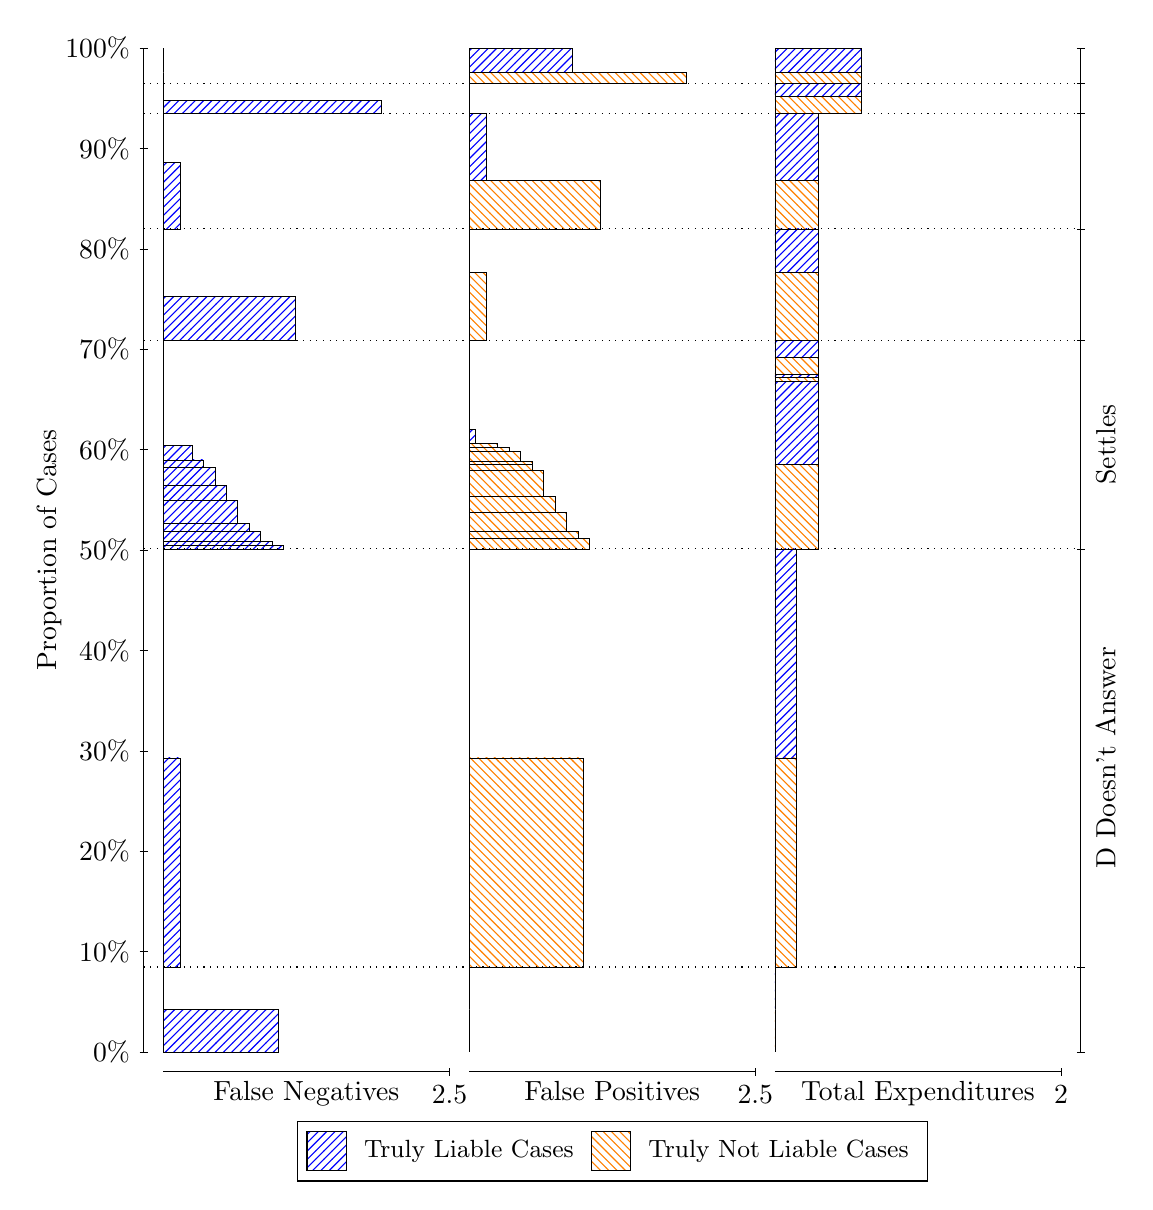
\begin{tikzpicture}
\draw[black, very thin] (1.5,1.75) -- (1.5,14.5);
\node[rotate=90, text=black, anchor=center] at (0.3, 8.125) {Proportion of Cases};
\draw[black, very thin] (1.45,1.75) -- (1.55,1.75);
\node[text=black, anchor=east] at (1.45, 1.75) {0\%};
\draw[black, very thin] (1.45,3.025) -- (1.55,3.025);
\node[text=black, anchor=east] at (1.45, 3.025) {10\%};
\draw[black, very thin] (1.45,4.3) -- (1.55,4.3);
\node[text=black, anchor=east] at (1.45, 4.3) {20\%};
\draw[black, very thin] (1.45,5.575) -- (1.55,5.575);
\node[text=black, anchor=east] at (1.45, 5.575) {30\%};
\draw[black, very thin] (1.45,6.85) -- (1.55,6.85);
\node[text=black, anchor=east] at (1.45, 6.85) {40\%};
\draw[black, very thin] (1.45,8.125) -- (1.55,8.125);
\node[text=black, anchor=east] at (1.45, 8.125) {50\%};
\draw[black, very thin] (1.45,9.4) -- (1.55,9.4);
\node[text=black, anchor=east] at (1.45, 9.4) {60\%};
\draw[black, very thin] (1.45,10.675) -- (1.55,10.675);
\node[text=black, anchor=east] at (1.45, 10.675) {70\%};
\draw[black, very thin] (1.45,11.95) -- (1.55,11.95);
\node[text=black, anchor=east] at (1.45, 11.95) {80\%};
\draw[black, very thin] (1.45,13.225) -- (1.55,13.225);
\node[text=black, anchor=east] at (1.45, 13.225) {90\%};
\draw[black, very thin] (1.45,14.5) -- (1.55,14.5);
\node[text=black, anchor=east] at (1.45, 14.5) {100\%};

\draw[black, very thin] (13.4,1.75) -- (13.4,14.5);
\draw[black, very thin] (13.35,1.75) -- (13.45,1.75);
\node[anchor=west] at (13.35, 1.75) {};
\draw[black, very thin] (13.35,2.8293) -- (13.45,2.8293);
\node[anchor=west] at (13.35, 2.8293) {};
\draw[black, very thin] (13.35,8.1397) -- (13.45,8.1397);
\node[anchor=west] at (13.35, 8.1397) {};
\draw[black, very thin] (13.35,10.79) -- (13.45,10.79);
\node[anchor=west] at (13.35, 10.79) {};
\draw[black, very thin] (13.35,12.204) -- (13.45,12.204);
\node[anchor=west] at (13.35, 12.204) {};
\draw[black, very thin] (13.35,13.666) -- (13.45,13.666);
\node[anchor=west] at (13.35, 13.666) {};
\draw[black, very thin] (13.35,14.054) -- (13.45,14.054);
\node[anchor=west] at (13.35, 14.054) {};
\draw[black, very thin] (13.35,14.5) -- (13.45,14.5);
\node[anchor=west] at (13.35, 14.5) {};

\draw[black, very thin, pattern color=blue, pattern=north east lines] (1.75,1.75) rectangle (3.2033,2.2896);
\draw[black, very thin, pattern color=orange, pattern=north west lines] (1.75,2.2896) rectangle (1.75,2.8293);
\draw[black, very thin, pattern color=blue, pattern=north east lines] (1.75,2.8293) rectangle (1.968,5.4845);
\draw[black, very thin, pattern color=orange, pattern=north west lines] (1.75,5.4845) rectangle (1.75,8.1397);
\draw[black, very thin, pattern color=blue, pattern=north east lines] (1.75,8.1397) rectangle (3.276,8.1804);
\draw[black, very thin, pattern color=blue, pattern=north east lines] (1.75,8.1804) rectangle (3.1307,8.2351);
\draw[black, very thin, pattern color=blue, pattern=north east lines] (1.75,8.2351) rectangle (2.9853,8.3609);
\draw[black, very thin, pattern color=blue, pattern=north east lines] (1.75,8.3609) rectangle (2.84,8.4664);
\draw[black, very thin, pattern color=blue, pattern=north east lines] (1.75,8.4664) rectangle (2.6947,8.7573);
\draw[black, very thin, pattern color=blue, pattern=north east lines] (1.75,8.7573) rectangle (2.5493,8.9434);
\draw[black, very thin, pattern color=blue, pattern=north east lines] (1.75,8.9434) rectangle (2.404,9.1763);
\draw[black, very thin, pattern color=blue, pattern=north east lines] (1.75,9.1763) rectangle (2.2587,9.2702);
\draw[black, very thin, pattern color=blue, pattern=north east lines] (1.75,9.2702) rectangle (2.1133,9.4499);
\draw[black, very thin, pattern color=orange, pattern=north west lines] (1.75,9.4499) rectangle (1.75,10.79);
\draw[black, very thin, pattern color=blue, pattern=north east lines] (1.75,10.79) rectangle (3.4213,11.343);
\draw[black, very thin, pattern color=orange, pattern=north west lines] (1.75,11.343) rectangle (1.75,12.204);
\draw[black, very thin, pattern color=blue, pattern=north east lines] (1.75,12.204) rectangle (1.968,13.048);
\draw[black, very thin, pattern color=orange, pattern=north west lines] (1.75,13.048) rectangle (1.75,13.666);
\draw[black, very thin, pattern color=blue, pattern=north east lines] (1.75,13.666) rectangle (4.5113,13.831);
\draw[black, very thin, pattern color=orange, pattern=north west lines] (1.75,13.831) rectangle (1.75,14.054);
\draw[black, very thin, pattern color=orange, pattern=north west lines] (1.75,14.054) rectangle (1.75,14.192);
\draw[black, very thin, pattern color=blue, pattern=north east lines] (1.75,14.192) rectangle (1.75,14.5);
\draw[black, very thin, pattern color=orange, pattern=north west lines] (5.6333,1.75) rectangle (5.6333,2.2896);
\draw[black, very thin, pattern color=blue, pattern=north east lines] (5.6333,2.2896) rectangle (5.6333,2.8293);
\draw[black, very thin, pattern color=orange, pattern=north west lines] (5.6333,2.8293) rectangle (7.0867,5.4845);
\draw[black, very thin, pattern color=blue, pattern=north east lines] (5.6333,5.4845) rectangle (5.6333,8.1397);
\draw[black, very thin, pattern color=orange, pattern=north west lines] (5.6333,8.1397) rectangle (7.1593,8.2719);
\draw[black, very thin, pattern color=orange, pattern=north west lines] (5.6333,8.2719) rectangle (7.014,8.3624);
\draw[black, very thin, pattern color=orange, pattern=north west lines] (5.6333,8.3624) rectangle (6.8687,8.605);
\draw[black, very thin, pattern color=orange, pattern=north west lines] (5.6333,8.605) rectangle (6.7233,8.8068);
\draw[black, very thin, pattern color=orange, pattern=north west lines] (5.6333,8.8068) rectangle (6.578,9.1362);
\draw[black, very thin, pattern color=orange, pattern=north west lines] (5.6333,9.1362) rectangle (6.4327,9.213);
\draw[black, very thin, pattern color=orange, pattern=north west lines] (5.6333,9.213) rectangle (6.4327,9.2473);
\draw[black, very thin, pattern color=orange, pattern=north west lines] (5.6333,9.2473) rectangle (6.2873,9.377);
\draw[black, very thin, pattern color=orange, pattern=north west lines] (5.6333,9.377) rectangle (6.142,9.4303);
\draw[black, very thin, pattern color=orange, pattern=north west lines] (5.6333,9.4303) rectangle (5.9967,9.4802);
\draw[black, very thin, pattern color=blue, pattern=north east lines] (5.6333,9.4802) rectangle (5.706,9.6599);
\draw[black, very thin, pattern color=blue, pattern=north east lines] (5.6333,9.6599) rectangle (5.6333,10.79);
\draw[black, very thin, pattern color=orange, pattern=north west lines] (5.6333,10.79) rectangle (5.8513,11.651);
\draw[black, very thin, pattern color=blue, pattern=north east lines] (5.6333,11.651) rectangle (5.6333,12.204);
\draw[black, very thin, pattern color=orange, pattern=north west lines] (5.6333,12.204) rectangle (7.3047,12.823);
\draw[black, very thin, pattern color=blue, pattern=north east lines] (5.6333,12.823) rectangle (5.8513,13.666);
\draw[black, very thin, pattern color=orange, pattern=north west lines] (5.6333,13.666) rectangle (5.6333,13.889);
\draw[black, very thin, pattern color=blue, pattern=north east lines] (5.6333,13.889) rectangle (5.6333,14.054);
\draw[black, very thin, pattern color=orange, pattern=north west lines] (5.6333,14.054) rectangle (8.3947,14.192);
\draw[black, very thin, pattern color=blue, pattern=north east lines] (5.6333,14.192) rectangle (6.9413,14.5);
\draw[black, very thin, pattern color=orange, pattern=north west lines] (9.5167,1.75) rectangle (9.5167,2.2896);
\draw[black, very thin, pattern color=blue, pattern=north east lines] (9.5167,2.2896) rectangle (9.5167,2.8293);
\draw[black, very thin, pattern color=orange, pattern=north west lines] (9.5167,2.8293) rectangle (9.7892,5.4845);
\draw[black, very thin, pattern color=blue, pattern=north east lines] (9.5167,5.4845) rectangle (9.7892,8.1397);
\draw[black, very thin, pattern color=orange, pattern=north west lines] (9.5167,8.1397) rectangle (10.062,9.213);
\draw[black, very thin, pattern color=blue, pattern=north east lines] (9.5167,9.213) rectangle (10.062,10.267);
\draw[black, very thin, pattern color=orange, pattern=north west lines] (9.5167,10.267) rectangle (10.062,10.317);
\draw[black, very thin, pattern color=blue, pattern=north east lines] (9.5167,10.317) rectangle (10.062,10.357);
\draw[black, very thin, pattern color=orange, pattern=north west lines] (9.5167,10.357) rectangle (10.062,10.575);
\draw[black, very thin, pattern color=blue, pattern=north east lines] (9.5167,10.575) rectangle (10.062,10.79);
\draw[black, very thin, pattern color=orange, pattern=north west lines] (9.5167,10.79) rectangle (10.062,11.651);
\draw[black, very thin, pattern color=blue, pattern=north east lines] (9.5167,11.651) rectangle (10.062,12.204);
\draw[black, very thin, pattern color=orange, pattern=north west lines] (9.5167,12.204) rectangle (10.062,12.823);
\draw[black, very thin, pattern color=blue, pattern=north east lines] (9.5167,12.823) rectangle (10.062,13.666);
\draw[black, very thin, pattern color=orange, pattern=north west lines] (9.5167,13.666) rectangle (10.607,13.889);
\draw[black, very thin, pattern color=blue, pattern=north east lines] (9.5167,13.889) rectangle (10.607,14.054);
\draw[black, very thin, pattern color=orange, pattern=north west lines] (9.5167,14.054) rectangle (10.607,14.192);
\draw[black, very thin, pattern color=blue, pattern=north east lines] (9.5167,14.192) rectangle (10.607,14.5);
\draw[black, dotted] (1.5,2.8293) -- (13.4,2.8293);
\draw[black, dotted] (1.5,8.1397) -- (13.4,8.1397);
\draw[black, dotted] (1.5,10.79) -- (13.4,10.79);
\draw[black, dotted] (1.5,12.204) -- (13.4,12.204);
\draw[black, dotted] (1.5,13.666) -- (13.4,13.666);
\draw[black, dotted] (1.5,14.054) -- (13.4,14.054);
\draw[black, very thin] (1.75,1.5) -- (5.3833,1.5);
\node[text=black, anchor=north] at (3.5667, 1.5) {False Negatives};
\draw[black, very thin] (5.3833,1.45) -- (5.3833,1.55);
\node[text=black, anchor=north] at (5.3833, 1.45) {2.5};

\draw[black, very thin] (5.6333,1.5) -- (9.2667,1.5);
\node[text=black, anchor=north] at (7.45, 1.5) {False Positives};
\draw[black, very thin] (9.2667,1.45) -- (9.2667,1.55);
\node[text=black, anchor=north] at (9.2667, 1.45) {2.5};

\draw[black, very thin] (9.5167,1.5) -- (13.15,1.5);
\node[text=black, anchor=north] at (11.333, 1.5) {Total Expenditures};
\draw[black, very thin] (13.15,1.45) -- (13.15,1.55);
\node[text=black, anchor=north] at (13.15, 1.45) {2};


\node[text=black, centered, rotate=90] at (13.72, 5.4845) {D Doesn't Answer};
\node[text=black, centered, rotate=90] at (13.72, 9.465) {Settles};





\draw (7.449999999999999,1.5) node[draw=none] (baseCoordinate) {};
\begin{scope}[align=center]
        \matrix[scale=0.5, draw=black, below=0.5cm of baseCoordinate, nodes={draw}, column sep=0.1cm]{
            \node[rectangle, draw, minimum width=0.5cm, minimum height=0.5cm, pattern color=blue, pattern=north east lines] {}; &
            \node[draw=none, font=\small, text=black] (B) {Truly Liable Cases}; &
            \node[rectangle, draw, minimum width=0.5cm, minimum height=0.5cm, pattern color=orange, pattern=north west lines] {}; &
            \node[draw=none, font=\small, text=black] (B) {Truly Not Liable Cases}; \\
            };
\end{scope}

\end{tikzpicture}
\end{document}